\section{Convex sets}
\subsection{Definitions}
\begin{definition}[Convex set]
    A set $C$ is a \emph{convex set} if every segment that connects two points in $C$ is in $C$. Formally:
    \begin{equation*}
        \forall x, y \in C, \forall \theta \in [0, 1], \quad \theta x + (1 - \theta) y \in C
    \end{equation*}
\end{definition}

\begin{example}
    Here are some examples of convex and non-convex sets:
    \begin{figure}[H]
        \centering
        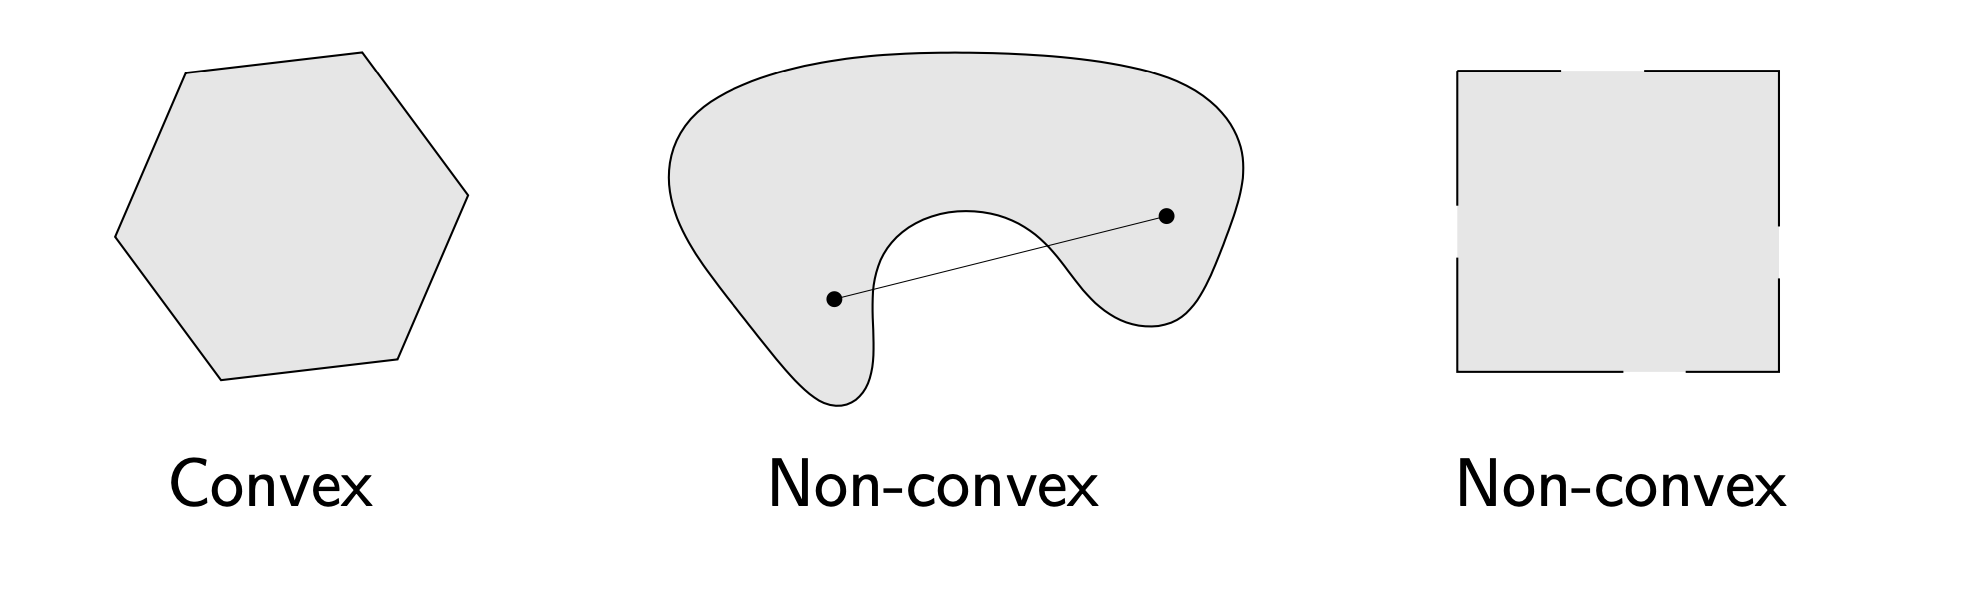
\includegraphics[width=.8\textwidth]{convex-sets/examples.png}
    \end{figure}
\end{example}
In many cases, we will use proper (i.e. non-empty) convex sets, and closed convex sets.

\begin{definition}[Convex hull]
    The \emph{convex hull} of $S$, denoted $\Conv(S)$, is the smallest convex set that contains $S$.
\end{definition}

\begin{definition}[Convex combinations]
    The \emph{convex combinations} of $x_1, \dots, x_k$ are all the point $x$ of the form:
    \begin{equation*}
        x = \theta_1x_1 + \dots + \theta_kx_k
    \end{equation*}
    with $\theta_1, \dots, \theta_k \geq 0$ and $\sum_{i=1}^k\theta_i = 1$.
\end{definition}

\begin{property}
    The convex hull of a set $S$ is the set of all convex combinations of points in $S$:
    \begin{equation*}
        \Conv(S) = \set{\sum_{i=1}^k\theta_ix_i}{(x_i)\in S^k, (\theta_i)\in\R_+^k, \sum_{i=1}^k\theta_i = 1}
    \end{equation*}
\end{property}

\subsection{Examples}
\subsubsection{Hyperplanes and halfspaces}
\begin{definition}[Hyperplane]
    A \emph{hyperplane} is the set of the form:
    \begin{equation*}
        H = \set{x}{a^\tp x = b}
    \end{equation*}
    for some $a\in\R^n\setminus\{0\}$ and $b\in\R$. $a$ is called the \emph{normal vector} of $H$. Hyperspaces are affine and convex.

    \begin{figure}[H]
        \centering
        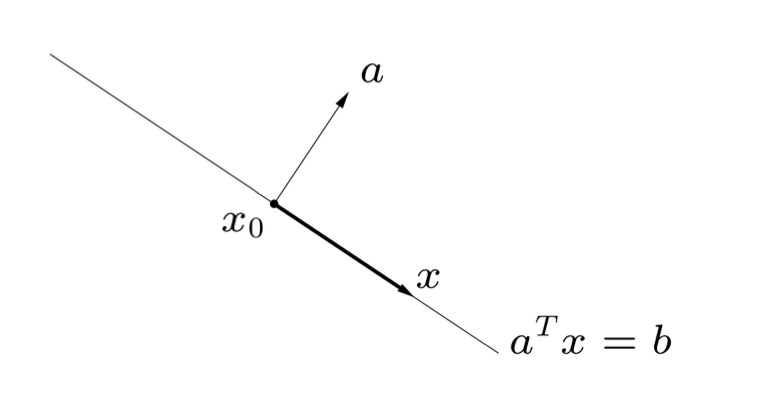
\includegraphics[width=.5\textwidth]{convex-sets/hyperplane.png}
        \caption{Hyperplane}
    \end{figure}
\end{definition}

\begin{definition}[Halfspace]
    A \emph{halfspace} is the set of the form:
    \begin{equation*}
        H = \set{x}{a^\tp x\leq b}
    \end{equation*}
    for some $a\in\R^n\setminus\{0\}$ and $b\in\R$. $a$ is called the \emph{normal vector} of $H$. Halfspaces are convex.

    \begin{figure}[H]
        \centering
        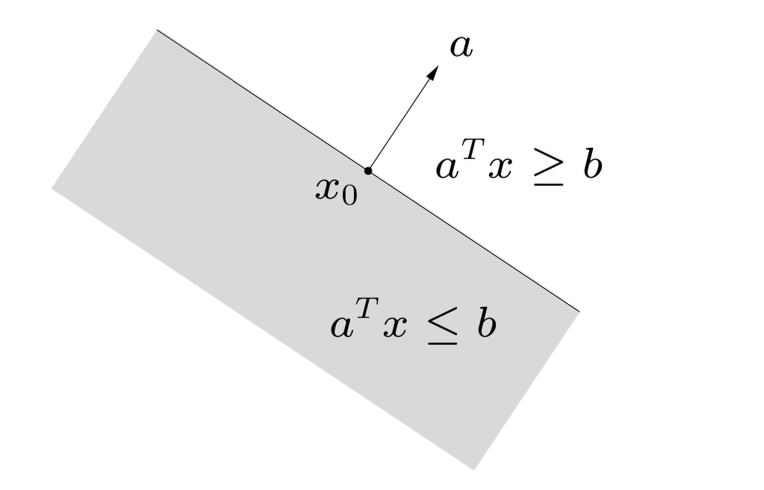
\includegraphics[width=.5\textwidth]{convex-sets/halfspace.png}
        \caption{Halfspace}
    \end{figure}
\end{definition}

\subsubsection{Euclidian balls and ellipsoids}
\begin{definition}[Euclidian ball]
    The \emph{Euclidian ball} of center $x_c$ and radius $r$ is the set:
    \begin{equation*}
        B(x_c, r) = \set{x}{\norm{x - x_c}_2\leq r} = \set{x_c+ru}{\norm{u}_2\leq 1}
    \end{equation*}
    Euclidian balls are convex.
\end{definition}

\begin{definition}[Ellipsoid]
    An \emph{ellipsoid} is the set of the form:
    \begin{equation*}
        E = \set{x}{(x - x_c)^\tp P^{-1}(x - x_c)\leq 1}
    \end{equation*}
    with $P\in\Sb^n_{++}$\footnote{$\Sb^n_{++}$ denotes the set of symmetric positive definite matrices of size $n$} and $x_c\in\R^n$. Ellipsoids are convex.

    \begin{figure}[H]
        \centering
        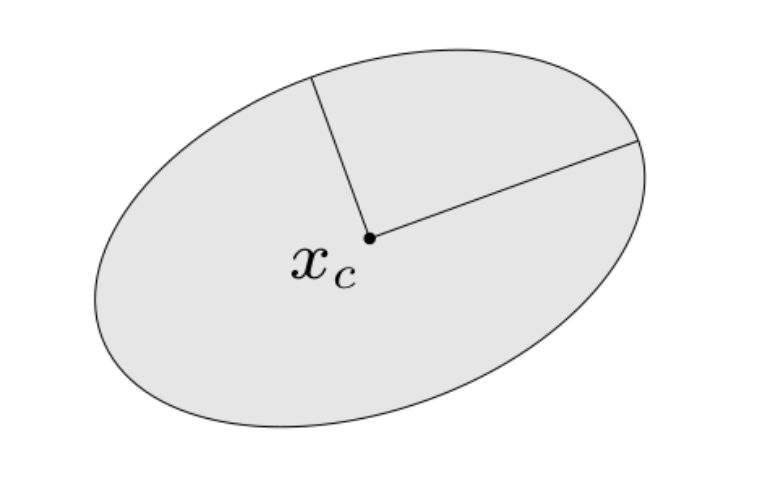
\includegraphics[width=.3\textwidth]{convex-sets/ellipsoid.png}
        \caption{Ellipsoid}
    \end{figure}

    An alternative representation of an ellipsoid is:
    \begin{equation*}
        E = \set{x_c + Au}{\norm{u}_2\leq 1}
    \end{equation*}
    for some nonsingular matrix $A\in\textnormal{GL}_n(\R)$. We can choose $A$ symmatric and positive definite without loss of generality, for instance by choosing $A = P^{1/2}$.
\end{definition}

\subsubsection{Cones}
\begin{definition}[Cones]
    A set $K$ is a \emph{cone}, or a \emph{nonnegative homogeneous set}, if:
    \begin{equation*}
        \forall x\in K, \forall \theta\in\R_+^*, \quad \theta x\in K
    \end{equation*}

    \begin{figure}[H]
        \centering
        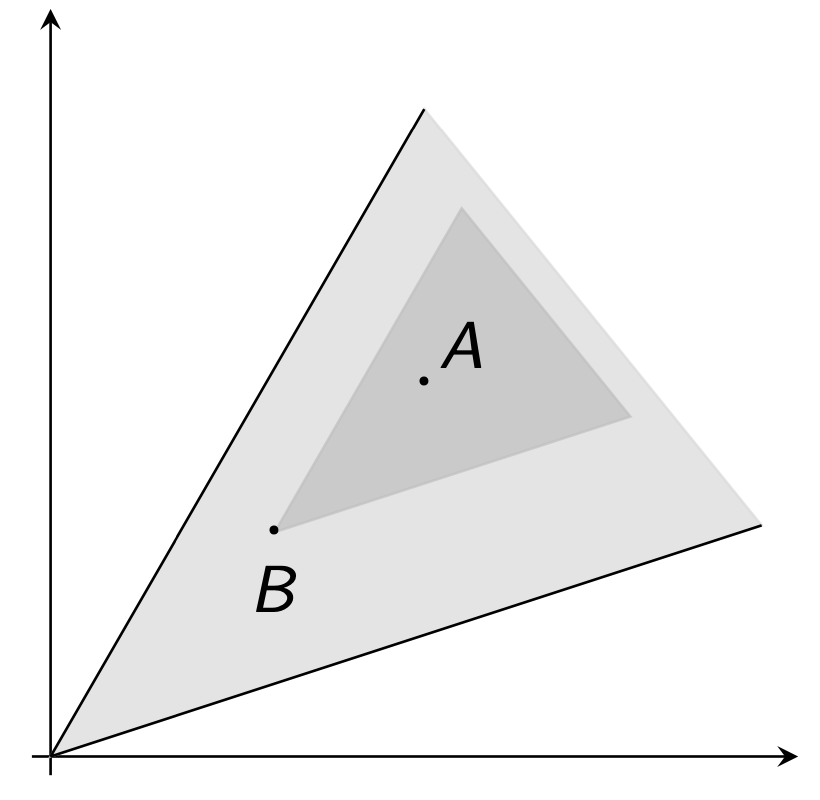
\includegraphics[width=.6\textwidth]{convex-sets/cone.png}
    \end{figure}
\end{definition}

\begin{definition}[Convex cone]
    A set $K$ is a \emph{convex cone} if:
    \begin{equation*}
        \forall x_1, x_2\in K, \forall \theta_1, \theta_2\in\R_+^*, \quad \theta_1x_1 + \theta_2x_2\in K
    \end{equation*}

    \begin{figure}[H]
        \centering
        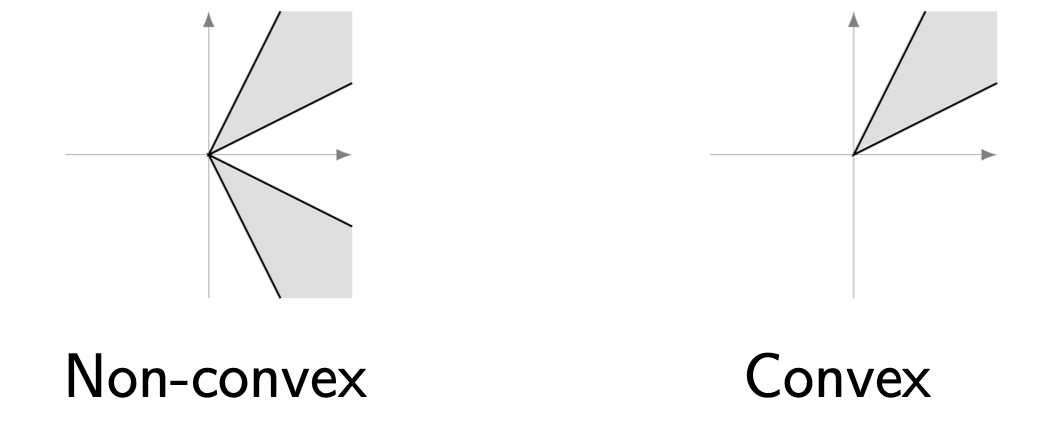
\includegraphics[width=.45\textwidth]{convex-sets/convex-cones.png}
    \end{figure}
\end{definition}

Special cases of cones include:
\begin{description}
    \item[Positive orthant] $K = \R_+^n = \set{x\in\R^n}{x_i\geq 0, \forall i}$
    \item[Norm cones] $K = \set{(x, t)\in\R^n\times\R}{\norm{x}\leq t}$. A particular case is the second-order cone (SOC), based on the $\ell_2$ norm.
    \item[Positive polynomials] $K_n = \set{x\in\R^{n+1}}{\forall t\in\R, \sum_{i=0}^n x_i t^i \geq 0}$
    \item[Positive semidefinite cone] $\Sb^n_+ = \set{X\in\Sb^n}{\forall z\in\R^n, z^\tp Xz\geq0}$ 
    \item[Co-positive cone] $\Sb^n_+ = \set{X\in\Sb^n}{\forall z\in\R^n_+, z^\tp Xz\geq0}$ 
    \item[Exponential cone] $\set{(x,y,z)\in\R\times\R_+^*\times\R}{z\geq ye^{x/y}}$ 
\end{description}

\subsection{Convexity-preserving operations}